\section{Gleichstrom-Schalter, Gleichstrom-Steller}
\subsection{nur Einschalten:}
  \begin{minipage}{0.5 \linewidth}
    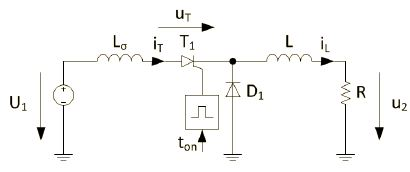
\includegraphics[width = \linewidth]{./pictures/gleichstromschalter}
  \end{minipage}
  \hfill
  \begin{minipage}{0.5 \linewidth}
    $L_{\sigma}$ ist die Streuinduktivität\\
    DGL nach der Zündung des Thyristors:\\
    $(L+L_{\sigma})\cdot \dfrac{di_{L}}{dt}+R\cdot i_{L}= U_{1}$\\
    $\rightarrow i_{L}(t)= \frac{U_{1}}{R}\cdot (1-e^{-\frac{t-t_{on}}{\tau}})$
  \end{minipage}

\subsection{Ein- und Ausschalten}

  \begin{minipage}{0.5 \linewidth}
    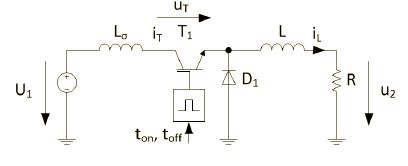
\includegraphics[width = \linewidth]{./pictures/gleichstromschalter2}
  \end{minipage}
  \hfill
  \begin{minipage}{0.5 \linewidth}
    $(L+L_{\sigma})\cdot \dfrac{di_{L}}{dt}+R\cdot i_{L}= U_{1},  t_{on} \leqslant t \leqslant t_{off}$\\
    $\rightarrow i_{L}(t)= \frac{U_{1}}{R}\cdot (1-e^{-\frac{t-t_{on}}{\tau}})$\\
    $(L+L_{\sigma})\cdot \dfrac{di_{L}}{dt}+R\cdot i_{L}= 0,  t \geqslant t_{off}$\\
    $\rightarrow i_{L}(t) = \frac{U_{1}}{R} \cdot e^{-\frac{t-t_{off}}{\tau}}$
  \end{minipage}

\subsection{Streuinduktivität}
Magnetfeld hat die Energie $W_{M} = \iiint H \cdot B dV $ \\
$\phi_{\sigma} = L_{\sigma}I_{t}^2, L_{\sigma}= \frac{2W_{M}}{i_{t}^2}$

\subsection{Gleichstromsteller (Chopper)}


  \begin{minipage}{0.5 \linewidth}
    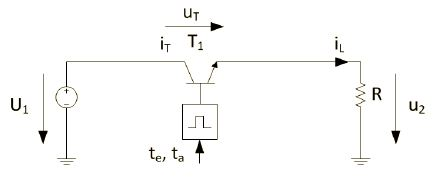
\includegraphics[width = \linewidth]{./pictures/gleichstromschalter3}
    der Mittelwert der Lastspannung ist:\\
    $U_{2 AV} = \frac{1}{T}\int_{0}^{T}u_{2}(t)\cdot dt= \frac{1}{t_{e}+t_{a}}\int_{0}^{t_{e}}U_{1}\cdot dt$\\
    $U_{2 AV} = \frac{t_{e}}{t_{e}+t_{a}}U_{1}= \frac{t_{e}}{T}U_{1}$
  \end{minipage}
  \hfill
  \begin{minipage}{0.5 \linewidth}
    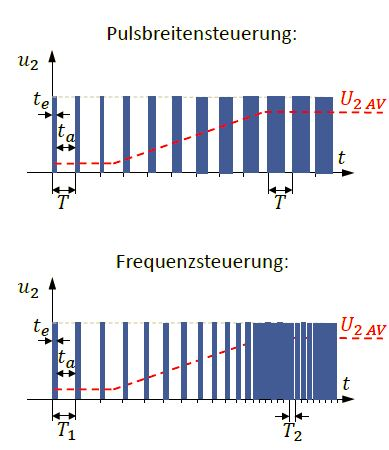
\includegraphics[width = \linewidth]{./pictures/gleichstromschalter4}
  \end{minipage}
